\documentclass{article}

\usepackage{amsmath,amssymb}
\usepackage{geometry}
\usepackage{graphicx}

\geometry{a4paper, margin=2.5cm}

\begin{document}

% ============================================================
\section*{GRPO and Verifiable Rewards (RLVR / Reinforcement Learning with Verifiable Rewards)}

\subsection*{First, a story}

All the trouble of the previous two chapters traces to a single source: the reward is a \textbf{learned} proxy from finitely covered preference data, and the gap between proxy and truth is amplified without bound by the optimizer. Yet many tasks need no learned reward at all --- whether a math answer is correct can be decided by one rule; whether code is correct, by running its tests.

\textbf{The naive approach}: train a reward model even for rule-scorable tasks. It will learn ``looks correct'' features and then get hacked by the optimizer --- the whole plot of Chapter 12 replays.

\textbf{This chapter's way}: if you can verify, don't learn. Use a rule-based verifier as the reward (correct $=1$, wrong $=0$), with a policy-gradient algorithm that needs no critic --- GRPO: sample a group of answers per prompt and use group-relative performance as the advantage.

\textbf{The core question}: once the reward cannot be hacked, what is the new bottleneck?

\[
\boxed{\hat{A}_{i} = \frac{r_{i} - \mathrm{mean}(r_{1},\dots,r_{G})}{\mathrm{std}(r_{1},\dots,r_{G})}}
\]

\subsection*{Formalization}

For each prompt $x$, sample $G$ completions $\{y_{i}\}_{i=1}^{G}$ from the current policy; the verifier assigns rewards $r_{i}=\mathrm{verify}(x, y_{i})\in\{0,1\}$. GRPO's objective is isomorphic to PPO, but the advantage is the within-group standardization:

\[
\boxed{J(\theta) = \mathbb{E}\left[\frac{1}{G}\sum_{i=1}^{G} \min\!\left(\rho_{i}\hat{A}_{i},\; \mathrm{clip}(\rho_{i}, 1\!-\!\epsilon, 1\!+\!\epsilon)\,\hat{A}_{i}\right)\right]}
\]

\begin{itemize}
  \item $\mathrm{verify}$ --- the rule-based verifier: exact match, unit tests, constraint checks; no learnable parameters;
  \item $G$ --- the group size, the number of samples per prompt; the group mean plays the prompt-specific baseline;
  \item $\rho_{i}$ --- the new-to-old policy probability ratio on completion $y_{i}$, as in Chapter 7's PPO-clip;
  \item $\hat{A}_{i}$ --- the group-relative advantage: no value network, normalized automatically by prompt difficulty.
\end{itemize}

% ============================================================
\section*{Task design: making the base model ``confidently wrong''}

The experiment uses two-digit addition: the prompt is ``d d + d d ='' and the model completes three digits; the reward is exact match. The key design is the SFT teacher: with probability $0.3$ it gives the correct answer, with $0.7$ the \textbf{digit-wise no-carry} answer. On carry prompts the wrong answer is the mode of the data --- the base model's greedy decoding has carry accuracy $0$: not noise but a \textbf{systematic wrong algorithm} baked in by SFT.

This is exactly the situation where learned rewards are helpless: a reward model trained on the same biased data would only learn ``no-carry'' as a high-scoring feature. The rule verifier looks at the answer, not the data: correct is correct. GRPO uses the roughly three-tenths correct rate surviving in the samples as signal, lifting overall accuracy from $0.30$ to $1.00$ within about 20 iterations, and carry accuracy from $0$ to $1.00$ (Figure~1).

\begin{figure}[!htbp]
  \centering
  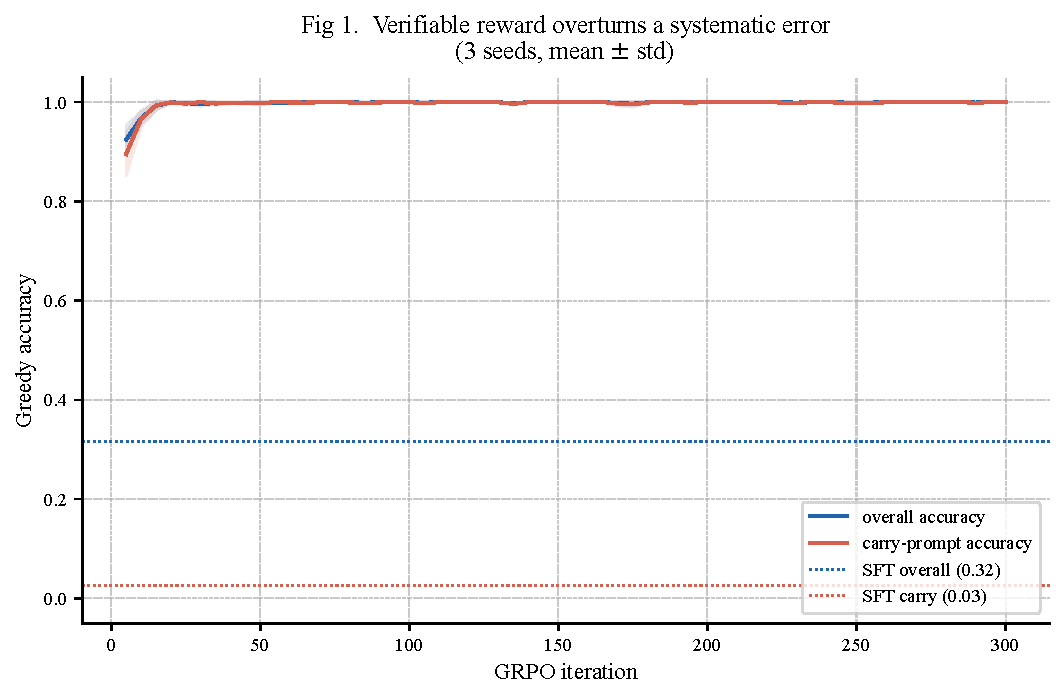
\includegraphics[width=0.88\textwidth]{fig1_rlvr_overturns.pdf}
  \caption{Verifiable reward overturns a systematic error (two-digit addition, 3 random seeds, shading $\pm 1\sigma$; dash-dotted lines, SFT baselines). The teacher ``cannot carry'': the SFT base model has overall accuracy $0.32$ and carry accuracy $0.03$; GRPO lifts both to $1.00$ within about 20 iterations.}
  \label{fig:grpo-overturn}
\end{figure}

% ============================================================
\section*{Core mechanisms}

\subsection*{Mechanism 1: the unhackable reward}

In Chapter 12, $\beta=0$ PPO pierces the learned reward within 60 iterations; in Chapter 13, DPO's soft anchor loosens with training. Here likewise $\beta=0$ for 600 long iterations: accuracy reaches the top and stays pinned; the KL to the reference holds at about $1$ nat (Figure~2).

The reason lies in the reward, not the algorithm: \textbf{the verifier and the true objective are the same function} --- there is no gap between proxy and truth for the optimizer to slip into; the harder the optimization, the more firmly it locks in correct answers. KL anchoring changes from necessity to option. The only remaining risk is whether the verifier itself has holes (answer-format bypasses, incomplete test suites) --- an engineering problem, no longer a learning problem.

\begin{figure}[!htbp]
  \centering
  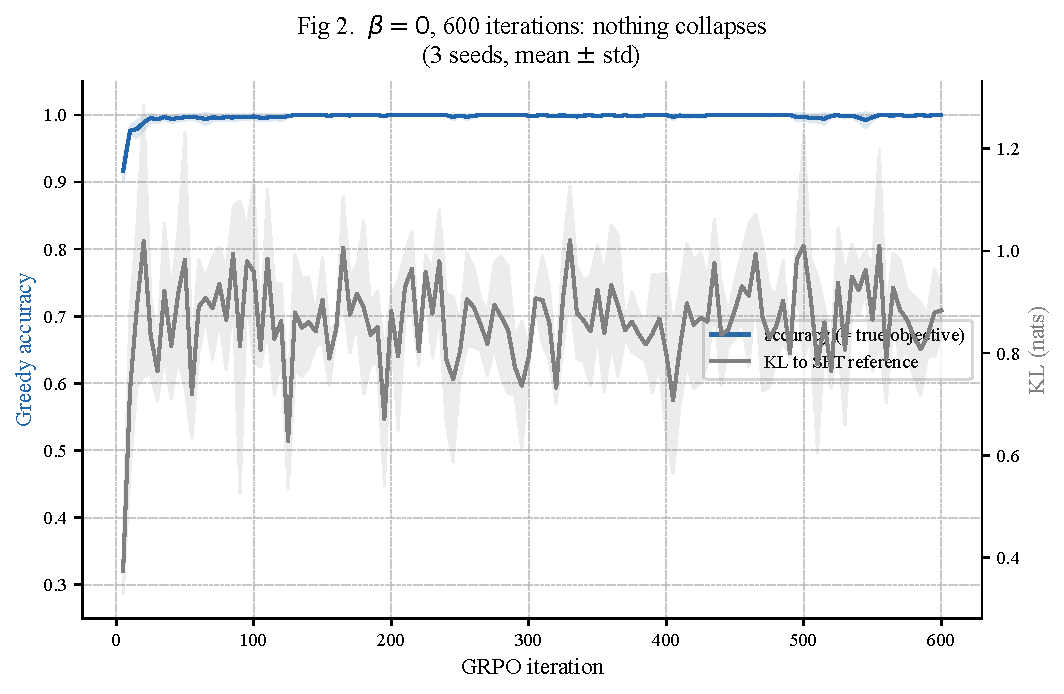
\includegraphics[width=0.88\textwidth]{fig2_unhackable_reward.pdf}
  \caption{$\beta=0$, 600 long iterations (3 random seeds, shading $\pm 1\sigma$). Accuracy (left axis) tops out and holds at $1.00$; KL (right axis) stays near $1$ nat --- contrast Chapter 12's $\beta=0$ collapse and Chapter 13's loosening anchor: with verifiable rewards, no anchor and no collapse.}
  \label{fig:grpo-unhackable}
\end{figure}

\subsection*{Mechanism 2: the group-relative baseline --- comparison instead of a critic}

PPO needs a value network for the baseline; GRPO replaces it with the within-group mean of ``one prompt, one group'': easy prompts are all-correct within the group, hard prompts all-wrong --- advantages normalize automatically by difficulty, with no extra network. The group mean is one more kind of baseline beside Chapter 7's global batch baseline (this chapter does not contrast the two; it focuses on group mechanics) --- whose distinctive behavior emerges in the next mechanism.

\subsection*{Mechanism 3: zero-signal groups --- the new bottleneck is signal}

Verifiable rewards are usually sparse 0/1. Group-relative advantages depend on \textbf{within-group differences}: groups that are all-correct or all-wrong have zero standard deviation, hence zero advantage and zero gradient. Swap the teacher for one never correct on carries ($q=0$): the cold-start model's sampling success rate on carry prompts is $\approx 0$, so every group is either all-correct (no-carry prompts) or all-wrong (carry prompts) --- the zero-signal fraction stays at $100\%$: learning never begins and accuracy stays at $0.30$ (Figure~3).

The same statistic tells a different story under the weak-teacher start: the zero-signal fraction rises from about three in ten to nearly $100\%$ because everything has been mastered --- ``graduation''. All-same groups have two meanings; only accuracy can tell them apart. That is why reasoning-model training needs cold-start SFT data and curricula: verifiable rewards solve ``reward reliability'' and leave the hard part to ``exploration and signal density''.

\begin{figure}[!htbp]
  \centering
  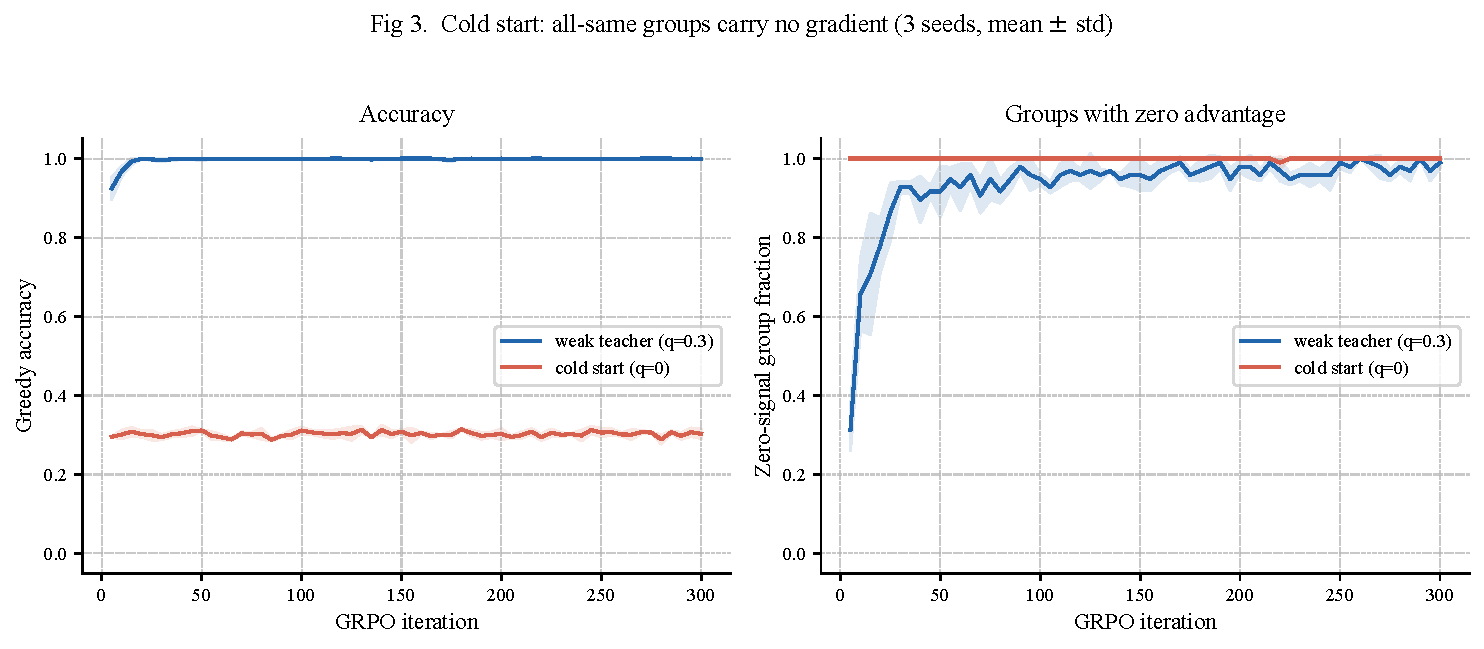
\includegraphics[width=0.88\textwidth]{fig3_cold_start.pdf}
  \caption{The death of cold start (3 random seeds, shading $\pm 1\sigma$). Left: the weak-teacher start (blue) rises to $1.00$; the cold start (red --- a teacher never correct on carries) stays at $0.30$. Right: the zero-signal group fraction --- cold start pinned at $100\%$ (all-same groups, zero gradient); the weak-teacher start climbs from about three in ten to nearly $100\%$ (mastered, graduated).}
  \label{fig:grpo-coldstart}
\end{figure}

% ============================================================
\section*{The full algorithm}

\subsection*{One GRPO iteration}

\begin{enumerate}
  \item \textbf{Sample}: take a batch of prompts; sample $G$ completions per prompt from the current policy;
  \item \textbf{Verify}: the rule verifier scores each $r_{i}\in\{0,1\}$;
  \item \textbf{Standardize within groups}: per prompt compute $\hat{A}_{i}=(r_{i}-\bar{r})/\mathrm{std}(r)$; all-same groups get zero advantage;
  \item \textbf{Update}: the PPO-clip objective with multi-epoch mini-batches; optionally add $-\beta\,\mathrm{KL}$ (this chapter's experiments use $\beta=0$).
\end{enumerate}

% ============================================================
\section*{GRPO vs PPO, RLVR vs RLHF}

\begin{itemize}
  \item \textbf{GRPO vs PPO}: drop the value network, replacing baseline estimation with within-group comparison --- one fewer model to train, at the cost of $G$ samples per prompt and dependence on within-group differences existing;
  \item \textbf{RLVR vs RLHF}: the reward source changes from ``human preference modeling'' to ``rule verification'' --- hacking the reward becomes impossible by construction, but applicability narrows to decidable tasks; the bottleneck shifts from reward reliability to reward sparsity and initial quality.
\end{itemize}

% ============================================================
\section*{Where this chapter sits in the RL landscape}

\begin{enumerate}
  \item Upstream: RLHF (Chapter 12) and DPO (Chapter 13) --- rewards learned from data, coverage sets the optimizable boundary;
  \item \underline{GRPO and verifiable rewards} (this chapter: if you can verify, don't learn --- the bottleneck shifts from reward to signal);
  \item Downstream: process rewards, curricula, and automatic verifier construction --- reshaping more tasks into ``verifiable'' form.
\end{enumerate}

Thus the trilogy closes. The reliability ranking of rewards is now clear: \textbf{rule verification $>$ human preference modeling $>$ hand design}. RLHF taught us that rewards can be learned but will be hacked; DPO taught us that skipping the component does not skip the coverage limit; RLVR taught us --- if you can verify, don't learn, and spend the effort on starting points, curricula and exploration.

\subsection*{References}

\begin{enumerate}
  \item Shao et al.\ (2024). DeepSeekMath: Pushing the Limits of Mathematical Reasoning in Open Language Models (GRPO). \textit{arXiv:2402.03300}.
  \item DeepSeek-AI (2025). DeepSeek-R1: Incentivizing Reasoning Capability in LLMs via Reinforcement Learning. \textit{arXiv:2501.12948}.
  \item Lambert et al.\ (2024). T\"ulu 3: Pushing Frontiers in Open Language Model Post-Training (RLVR). \textit{arXiv:2411.15124}.
  \item Schulman et al.\ (2017). Proximal Policy Optimization Algorithms. \textit{arXiv:1707.06347}.
\end{enumerate}

\end{document}
